\section{Abbildungs- und Tabellenverzeichnis erstellen}

In einer größeren, komplexen Arbeit, wie ein Fachbuch, hat man wahrscheinlich Tabellen und die eine oder andere Abbildung. Wenn man für diese eigene Verzeichnisse erstellen möchte, gibt es in Latex dafür passende Befehle. Diese Befehle sind \\listoffigures und \\listoftables. Damit die Befehle auch etwas zeigen, werden ein Bild und eine Tabelle gezeigt. Die beiden Befehle schreibt man in die Präambel.

\subsection{Abbildungen}

\subsubsection{Bitmap-Grafiken platzieren}

Abbildungen sind ein wesentlicher Bestandteil von Sach- und Fachbüchern, sowie von Sach- und Fachartikeln. Sie lockern lange Textpassagen auf und veranschaulichen Zusammenhänge.

Für dieses Beispiel wird eine Bitmap-Grafik eingebunden und verschieden platziert. Als erstes soll das Bild in Originalgröße zentriert eingebunden werden.

\begin{figure}[H]
	\centering
	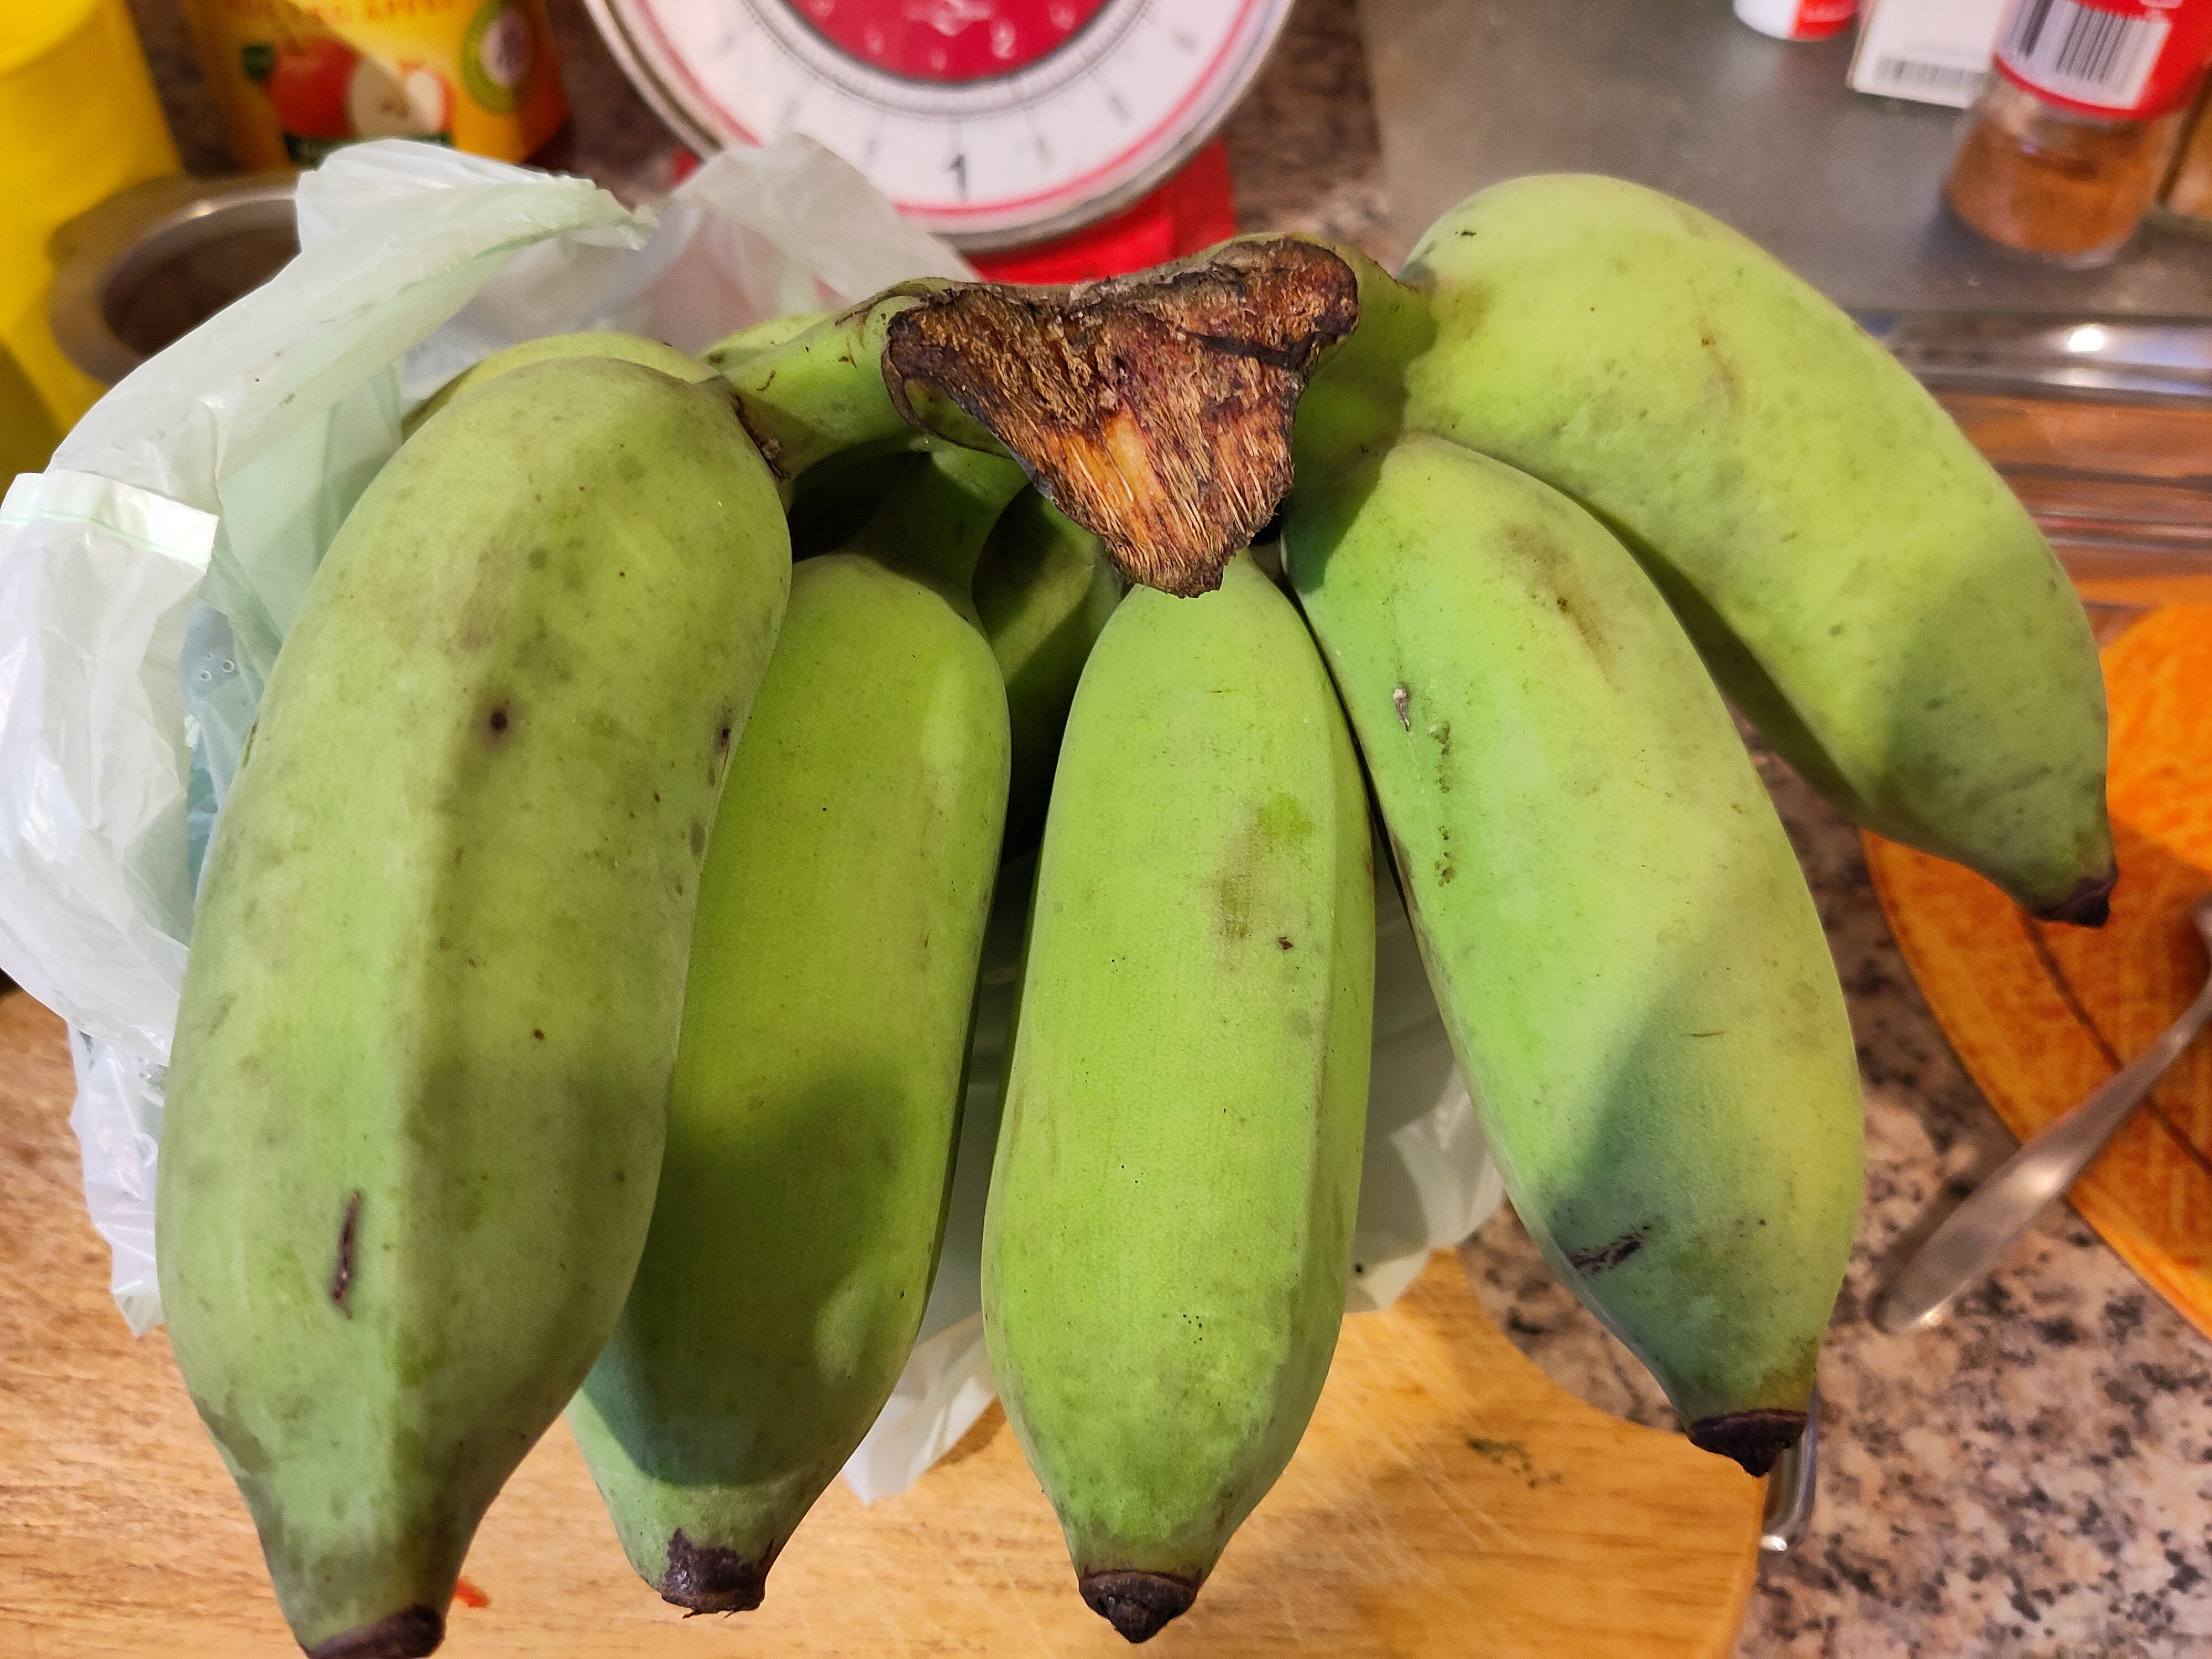
\includegraphics[width=0.95\textwidth]{../images/ThaiBananen}
	\caption{Unreife Bananen aus Thailand -- Originalgröße}
	\label{fig:thai-bananen}
	\end{figure}
	
Mit der Angabe der Breite gibt man an, wieviel Prozent des Papiers das Bild in Anspruch nehmen soll, abzüglich der Seitenränder. 1.0 entspricht hierbei 100 \%, also die gesamte Breite. In diesem Beispiel wurde eine Breite von 0.95 gewählt, damit das Bild an beiden Rändern ein wenig eingerückt wird.

Im nächsten Beispiel soll das Bild auf der linken Seite eingebunden werden.


		
